\documentclass[ngerman]{scrreprt}
\usepackage{babel}
\usepackage{blindtext}
\usepackage{microtype}
\usepackage{booktabs}
\usepackage{graphicx}

\author{Uwe Ziegenhagen}
\title{Mein zweites \LaTeX-Dokument}
\date{Köln, den \today}

\usepackage{hyperref}
\hypersetup{
    bookmarks=true,                     % show bookmarks bar
    unicode=false,                      % non - Latin characters in Acrobat’s bookmarks
    pdftoolbar=true,                        % show Acrobat’s toolbar
    pdfmenubar=true,                        % show Acrobat’s menu
    pdffitwindow=false,                 % window fit to page when opened
    pdfstartview={FitH},                    % fits the width of the page to the window
    pdftitle={My title},                        % title
    pdfauthor={Author},                 % author
    pdfsubject={Subject},                   % subject of the document
    pdfcreator={Creator},                   % creator of the document
    pdfproducer={Producer},             % producer of the document
    pdfkeywords={keyword1, key2, key3},   % list of keywords
    pdfnewwindow=true,                  % links in new window
    colorlinks=true,                        % false: boxed links; true: colored links
    linkcolor=blue,                          % color of internal links
    filecolor=blue,                     % color of file links
    citecolor=blue,                     % color of file links
    urlcolor=blue                        % color of external links
}

\begin{document}
\maketitle

\tableofcontents

\listoftables

\listoffigures

\chapter{Einleitung}
\section{Einführung}
\subsection{Literatur}
\subsection{Handelnde Personen}

\blindtext

\captionof{table}{Hallo, ich bin die Tabelle}\label{tab:erstetab}
\begin{tabular}{|l|c|r|p{8cm}|} \hline
sp1z1 & sp2z1 & sp3z1 & sp4z1 \\ \hline
345324532etr  & 235342323434 & 534 & Hallo  \\ \hline
\end{tabular}


\begin{center}
\captionof{table}{Hallo, ich bin die booktabsTabelle}\label{tab:erstebooktab}
\begin{tabular}{lcrp{4cm}} \toprule[2.5pt]
\textbf{sp1z1} & \textbf{sp2z1} & \textbf{sp3z1} & \textbf{sp4z1} \\ \addlinespace \cmidrule(rl){1-3}
345324532etr  & 235342323434 & 534 & Hallo  \\ 
345324532etr  & 235342323434 & 534 & Hallo  \\ 
345324532etr  & 235342323434 & 534 & Hallo  \\ 
345324532etr  & 235342323434 & 534 & Hallo  \\ \bottomrule[5pt]
\end{tabular}
\end{center}


\clearpage

\begin{center}
\captionof{table}{Hallo, ich bin die Tabelle}
\label{tab:ertsebooktab}
\begin{tabular}{lcrp{2cm}}\toprule
\textbf{sp1z1} & \textbf{sp2z1} & \textbf{sp3z1} & \textbf{sp4Z1} \\ \midrule
34524532 & 23534234 & 43534 & Hallo\\
34524532 & 23534234 & 43534 & Hallo\\
34524532 & 23534234 & 43534 & Hallo\\
34524532 & 23534234 & 43534 & Hallo\\
\bottomrule
\end{tabular}
\end{center}

Siehe Tabelle \ref{tab:erstetab} auf Seite \pageref{tab:erstetab}.

\begin{center}
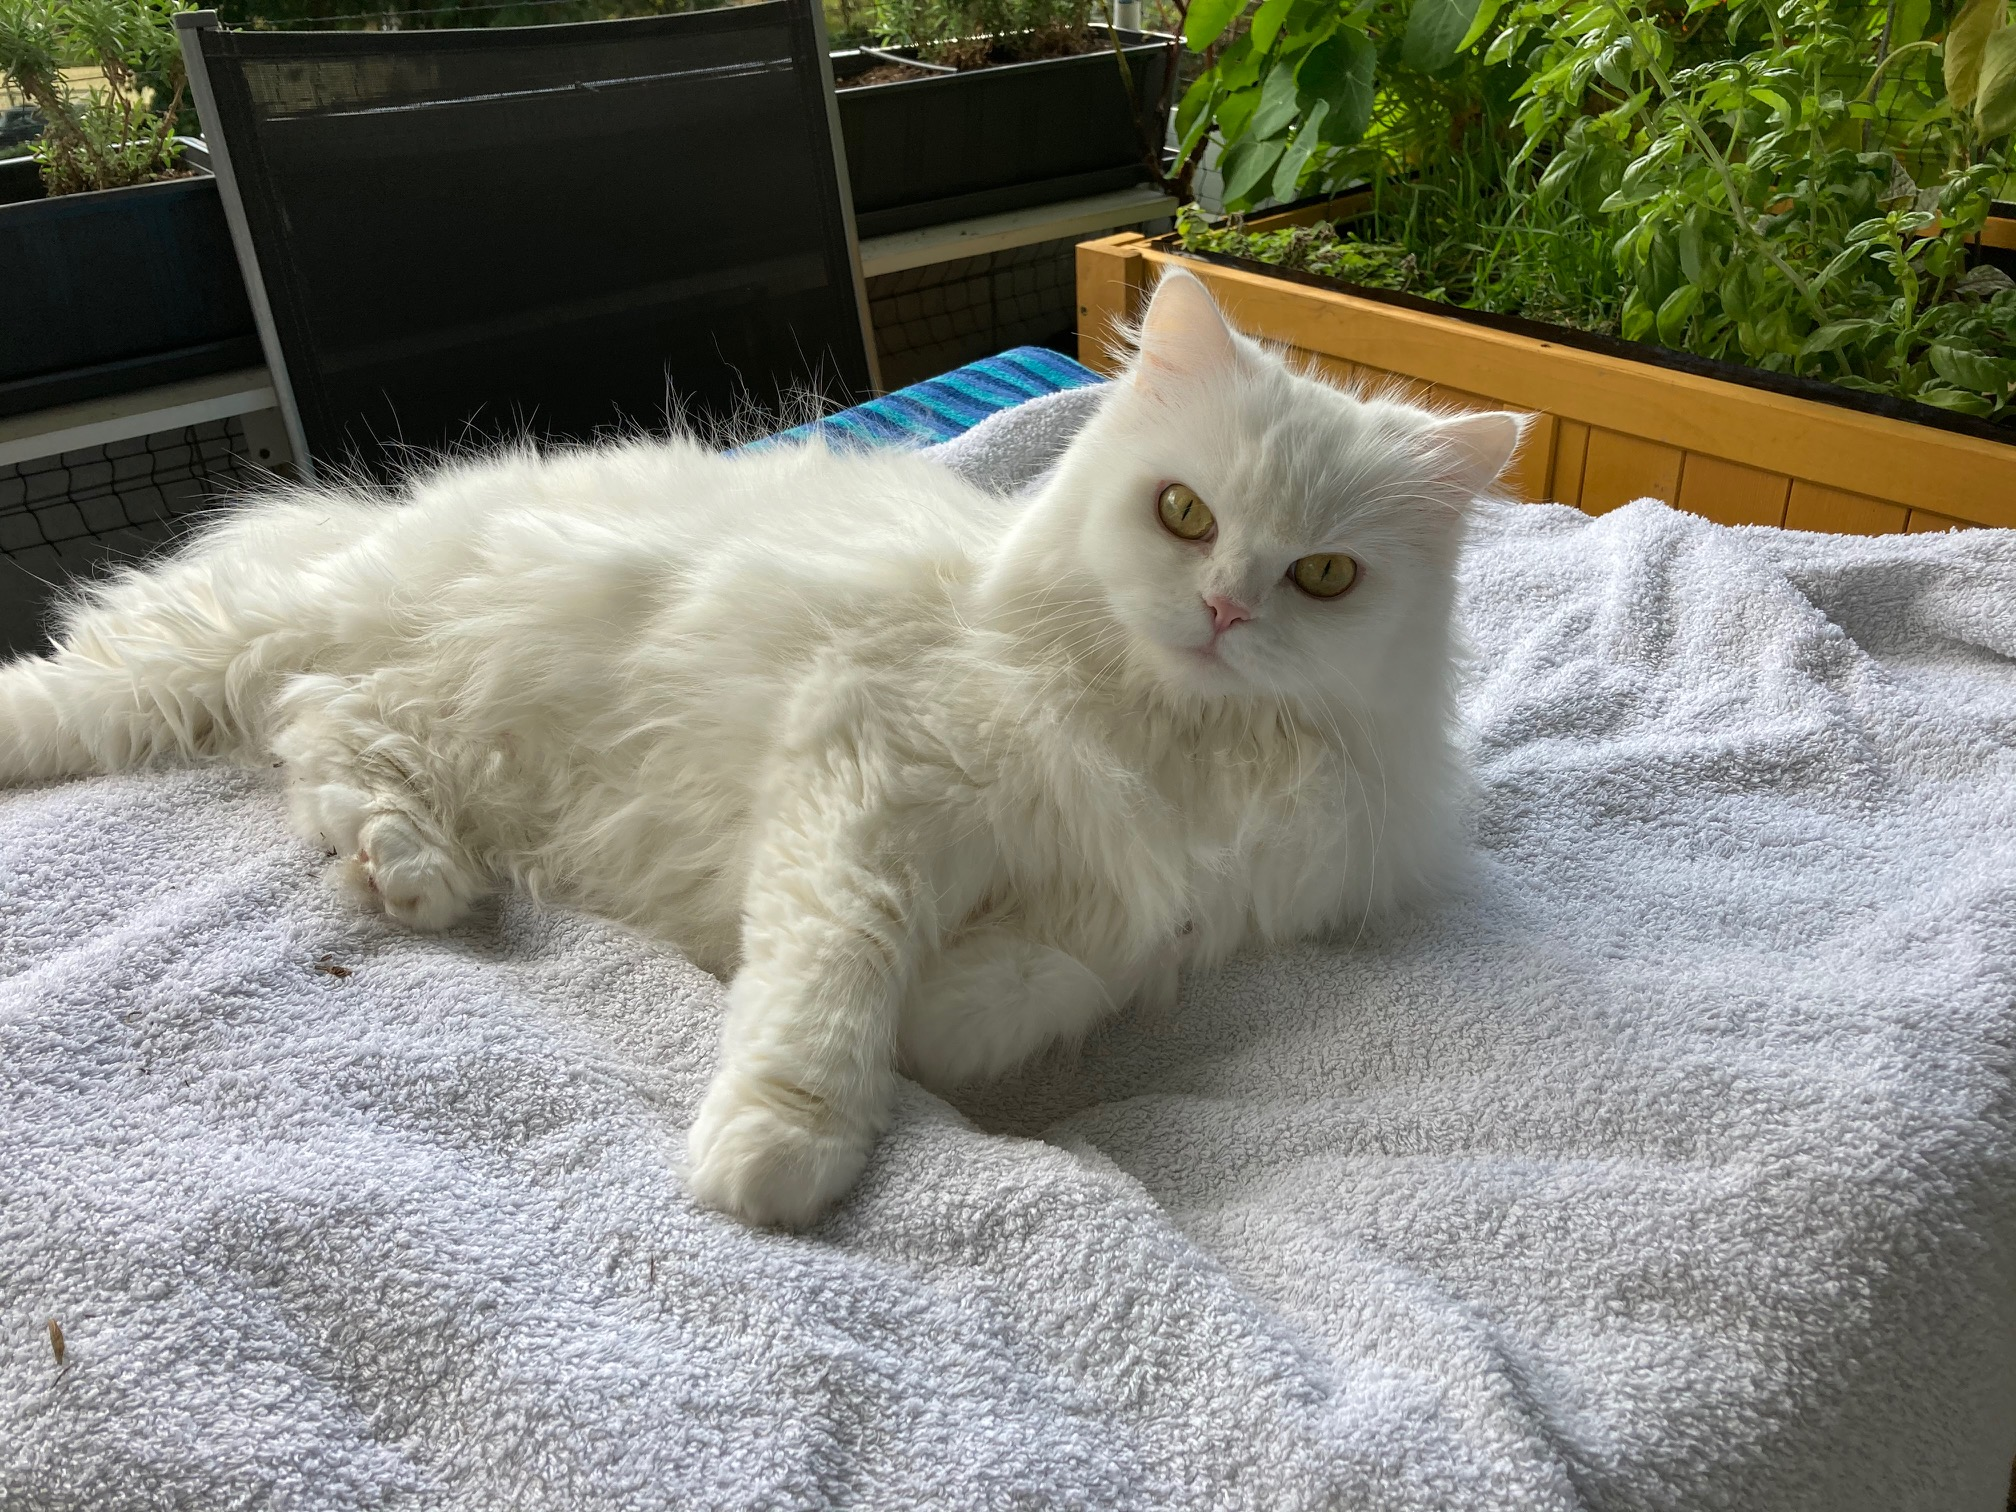
\includegraphics[width=0.8\textwidth]{Bilder/Katze1}
\captionof{figure}{Miezekatze auf dem Handtuch}
\end{center}


\end{document}

